\section{Background and Related Work}
\label{sec2}

\subsection{Background}

\begin{figure*}[!t]
    \centering
    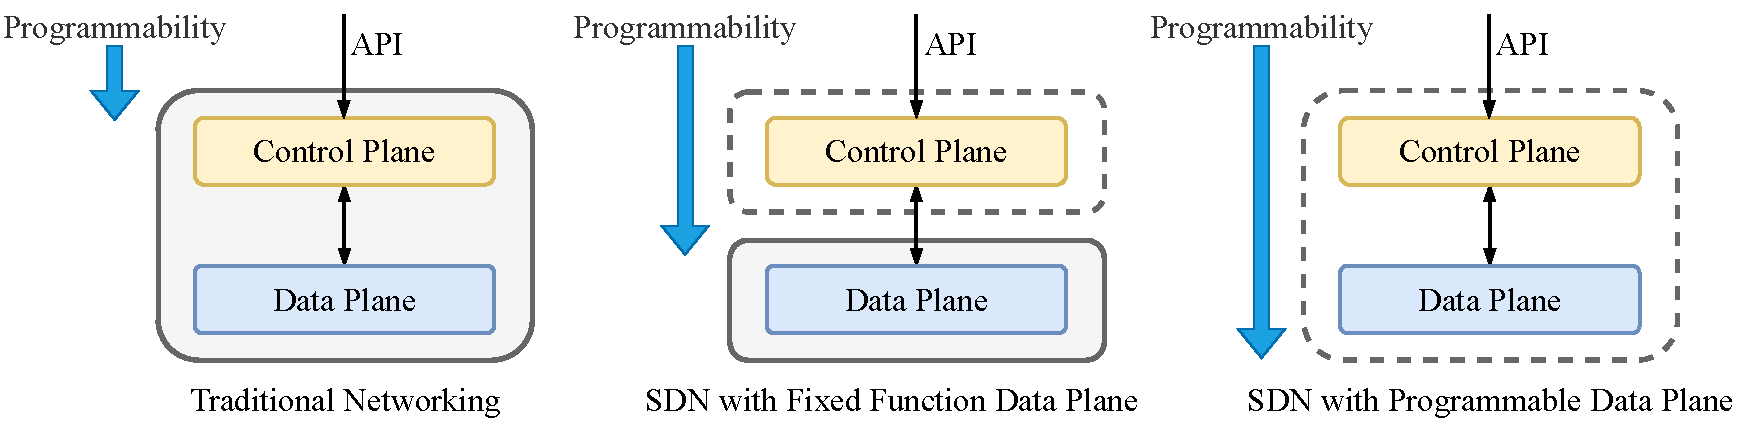
\includegraphics[width=0.85\textwidth]{./figures/evolution.pdf}
    \caption{Evolution of networks.}
    \label{evolution}
\end{figure*}

\noindent
% In recent years, network architectures have undergone a fundamental evolution, progressing from traditional distributed device management to centralized SDN, and further toward next-generation paradigms featuring programmable data planes. 
\rev{In recent years, network architectures have undergone a fundamental evolution, shifting from traditional distributed device management to centralized SDN, and further toward next-generation paradigms with programmable data planes.} 
This evolution is illustrated in Figure~\ref{evolution}. 
On the left of this figure, traditional network designs exhibit a tightly coupled relationship between the control logic and data forwarding processes. 
Network devices in this model are typically closed and inflexible, with static functions hardcoded by vendors. 
Updating policies requires manual intervention and device reconfiguration, significantly limiting the scalability and adaptability of the network. 
The middle part of the figure depicts the canonical SDN architecture, where the control plane is decoupled from individual network devices and centralized within the SDN controller(s). 
This architectural shift enables centralized policy management and dynamic control of network behavior, leading to substantial improvements in programmability and automation. However, this programmability is largely confined to the control plane. 
The data plane, constrained by static match-action rules, lacks the flexibility to respond rapidly and granularly to real-time traffic dynamics. 
The right part of the figure illustrates the integration of programmable data planes into SDN, marking a new phase in the evolution toward intelligent and highly customizable networks. 
By enabling programmability at the data plane, network devices can be redefined to support protocol-independent, state-aware, and fully customizable packet processing behaviors. 
This capability enhances the network's responsiveness to dynamic traffic patterns and significantly improves operational agility and efficiency.

A key technological milestone in this evolution is the emergence of the P4 language \cite{P4.org}, which plays a foundational role in the development of programmable data planes. 
P4 is a high-level, domain-specific language tailored for describing packet-processing behaviors. 
Its core design objective is to achieve protocol independence and flexible behavior specification within the data plane. 
% Using P4 programs, developers gain fine-grained control over the packet processing pipeline of a switch, including parsing, matching, modifying, and forwarding actions. 
\rev{P4 programs provide developers with fine-grained control over the packet processing pipeline of a switch, including parsing, matching, modifying, and forwarding actions.} 
This programmability not only extends the functional boundaries of network devices but also introduces new opportunities for building efficient and intelligent traffic monitoring systems. 
In particular, P4 facilitates the deployment of custom traffic classification and filtering mechanisms directly within the data plane. 
Developers can embed user-defined logic to monitor or tag only specific types of flows, thereby enabling preliminary state processing without relying on frequent controller intervention. 
Compared to traditional polling-based monitoring approaches, this architecture significantly reduces control plane communication overhead while improving response latency and system scalability.

\subsection{Related Work}

\noindent With the advancement of programmable data plane technologies, a variety of P4-based SDN traffic monitoring solutions have been proposed to improve the timeliness, accuracy, and scalability of network monitoring. 
Among them, In-band Network Telemetry (INT)~\cite{INT} represents a widely adopted monitoring framework. 
% The core idea of INT is to attach metadata to packet headers, which can be modified by intermediate switches along the forwarding path, enabling data plane state collection without controller intervention \cite{8094182, kim2015band}. 
\rev{The core idea of INT is to attach metadata to packet headers that are modified by intermediate switches along the forwarding path, enabling data plane state collection without controller intervention \cite{8094182, kim2015band}.} 
This mechanism allows switches to embed performance indicators such as latency and packet loss rate at each hop. 
The receiver subsequently extracts the full path metadata for comprehensive analysis. 
However, the additional headers introduced by INT result in significant protocol overhead, which increases sharply with path length and severely limits its practical applicability. 
To address this issue, researchers have developed several lightweight optimization strategies. 
For example, FS-INT \cite{SUH202062} proposes a flexible sampling mechanism that combines proportional and event-driven sampling to annotate only selected key packets with INT metadata. 
This approach retains essential monitoring capabilities while effectively controlling overhead, adapting to the performance requirements of diverse network environments. 
More recently, DLINT and PLINT \cite{10206040} have been proposed as deterministic and probabilistic enhancements to P4-INT. 
DLINT introduces per-flow telemetry state aggregation with Bloom filter-based compression, while PLINT adopts reservoir sampling to probabilistically embed telemetry information across packets. 
Both techniques significantly reduce overhead while preserving telemetry accuracy, offering complementary advantages in path trace reconstruction and update detection.

Beyond INT-based solutions, various active or distributed P4-enabled monitoring schemes have been developed. 
The network is partitioned into multiple monitoring domains by FlowStalker, where each domain collects local traffic information using specially crafted packets and periodically reports it to the controller \cite{8761197}. 
FlowSpy, in contrast, employs a load balancing mechanism to optimize communication between the data plane and controller, thereby enhancing monitoring efficiency \cite{8891487}. 
The work in \cite{9040030} explores pre-processing of monitoring data within switches, transmitting only essential information to alleviate control channel congestion. 
In addition, \cite{8967165} analyzes how the deployment of programmable switches affects monitoring performance and proposes optimized deployment strategies to improve system observability. 
Furthermore, the Time-based Sliding Window (TBSW) algorithm \cite{8855399} exploits the pipelined processing capabilities of P4 data planes to perform per-packet statistics over time-based windows. This significantly improves measurement accuracy while maintaining high processing efficiency. 
The algorithm has been prototyped on Barefoot Tofino ASIC (Application-Specific Integrated Circuit)~\cite{ASIC} hardware, demonstrating strong engineering feasibility. 

In the context of security, P4 has also been leveraged to enhance in-network threat detection and response. 
The study in \cite{9482549} utilizes P4-based flow feature extraction to support the controller in identifying potential threats and activating dynamic response mechanisms. 
Similarly, P4-MACsec \cite{9044731} implements link-layer encryption and integrity protection, strengthening communication security among programmable switches. 

A different approach is presented in \cite{10623873}, which introduces a hybrid monitoring paradigm known as PPM. 
This method integrates proactive reporting with distributed processing. 
Specifically, when certain monitoring metrics (e.g., accumulated byte or packet counts) for a flow exceed predefined thresholds, switches autonomously trigger reporting actions, eliminating reliance on controller-side polling. 
The PPM framework offers a promising direction for building low-overhead, high-accuracy intelligent monitoring systems on top of programmable data planes.

Compared to the aforementioned approaches, the method proposed in this study distinguishes itself by introducing a machine learning-driven adaptive threshold control mechanism into the P4-based monitoring pipeline. 
% As far as is known, this is the first monitoring framework to jointly leverage programmable data plane capabilities for event-driven data collection and control plane intelligence for real-time threshold optimization. 
\rev{This study presents the first monitoring framework that combines programmable data plane capabilities for event-driven data collection with control plane intelligence for real-time threshold optimization.} 
While prior works such as PPM rely on static or manually configured thresholds, the present method employs learned models to dynamically adjust monitoring parameters based on traffic context. 
This enables trade-offs between accuracy and overhead, which are difficult to achieve through rule-based or statically configured strategies alone.
